\subsection{Ursache-Wirkungs-Diagramm (Ishikawa) \hfill IP}
    \begin{scriptsize}
        \begin{itemize}
            \item \textbf{A.k.a:} Fischgrätendiagramm
            \item \textbf{Informelle Methode:} 1. Im Team exakte Beschreibung erarbeiten / 2. Problem-\\ursachen mittels Brainstorming erarbeiten / 3. Problemursachen Kategorien \\zuordnen
            \item \textbf{Hilft bei folgenden Aktivitäten:} Problem finden / Bestimmung der beteiligten \\Einflussgrössen / Auswahl der wichtigsten Faktoren / Untersuchung der Faktoren \\/ Beziehung zwischen Faktoren prüfen / Erzeugung und Strukturierung von Ideen
        \end{itemize}
    \end{scriptsize}
        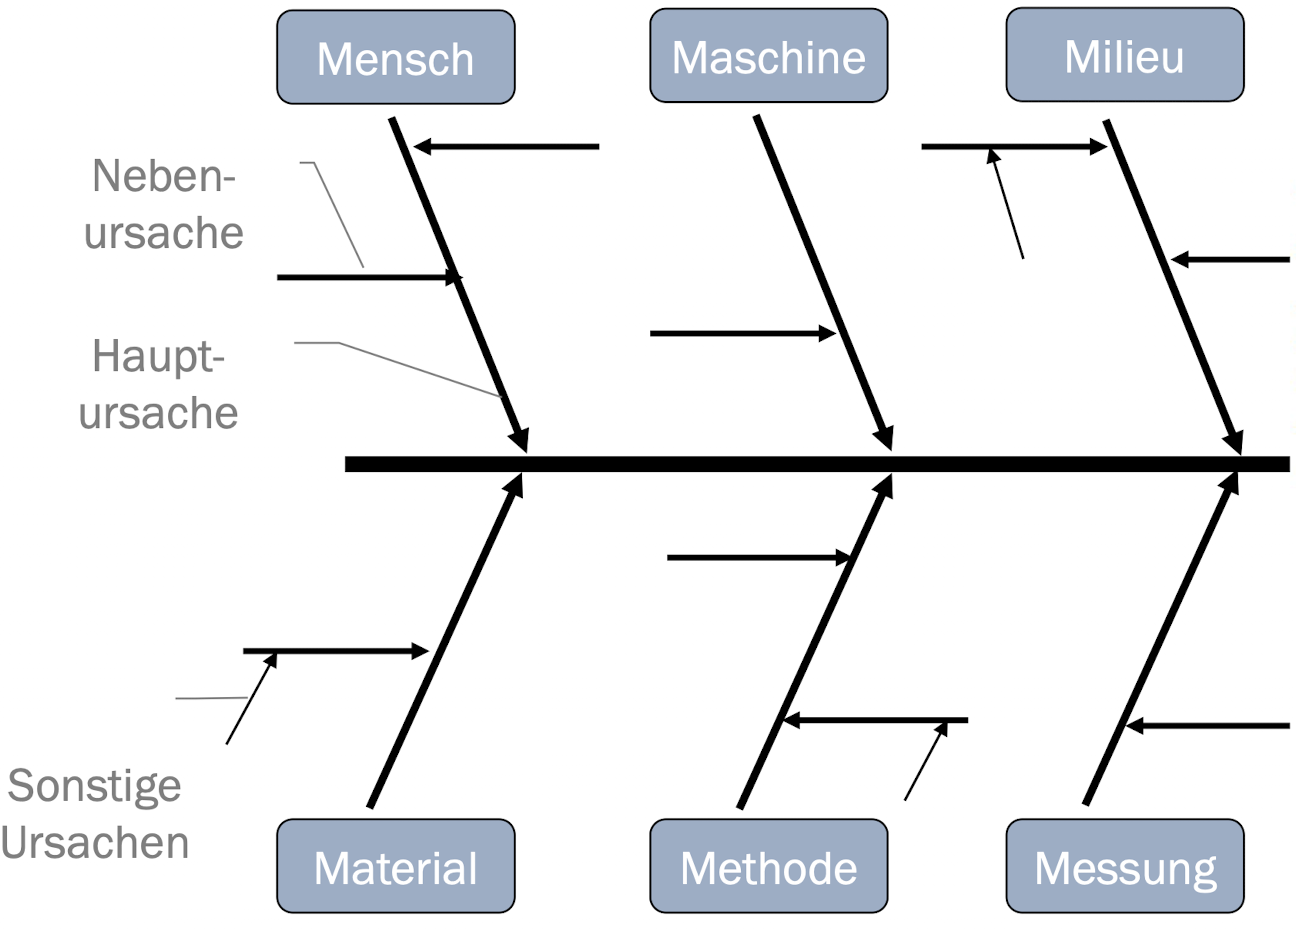
\includegraphics[width = 0.5\linewidth]{src/images/MAEIP_Fischgraeten}